%%%%%%%%%%%%%%%%%%%%%%%%%%%%%%%%%%%%%%%%%
% Stylish Article
% LaTeX Template
% Version 2.2 (2020-10-22)
%
% This template has been downloaded from:
% http://www.LaTeXTemplates.com
%
% Original author:
% Mathias Legrand (legrand.mathias@gmail.com)
% With extensive modifications by:
% Vel (vel@latextemplates.com)
%
% License:
% CC BY-NC-SA 3.0 (http://creativecommons.org/licenses/by-nc-sa/3.0/)
%
%%%%%%%%%%%%%%%%%%%%%%%%%%%%%%%%%%%%%%%%%

%----------------------------------------------------------------------------------------
%	PACKAGES AND OTHER DOCUMENT CONFIGURATIONS
%----------------------------------------------------------------------------------------

\documentclass[fleqn,10pt]{SelfArx} % Document font size and equations flushed left

\usepackage[english]{babel} % Specify a different language here - english by default
\usepackage{pgfgantt}

\usepackage{lipsum} % Required to insert dummy text. To be removed otherwise

%----------------------------------------------------------------------------------------
%	COLUMNS
%----------------------------------------------------------------------------------------

\setlength{\columnsep}{0.55cm} % Distance between the two columns of text
\setlength{\fboxrule}{0.75pt} % Width of the border around the abstract

%----------------------------------------------------------------------------------------
%	COLORS
%----------------------------------------------------------------------------------------

\definecolor{color1}{RGB}{0,0,90} % Color of the article title and sections
\definecolor{color2}{RGB}{0,20,20} % Color of the boxes behind the abstract and headings

%----------------------------------------------------------------------------------------
%	HYPERLINKS
%----------------------------------------------------------------------------------------

\usepackage{hyperref} % Required for hyperlinks

\usepackage{makecell}
\hypersetup{
	hidelinks,
	colorlinks,
	breaklinks=true,
	urlcolor=color2,
	citecolor=color1,
	linkcolor=color1,
	bookmarksopen=false,
	pdftitle={Title},
	pdfauthor={Author},
}

%----------------------------------------------------------------------------------------
%	ARTICLE INFORMATION
%----------------------------------------------------------------------------------------

\JournalInfo{Laboratory of biological data mining} % Journal information
\Archive{Project proposal} % Additional notes (e.g. copyright, DOI, review/research article)

\PaperTitle{Identification and validation of a vitamin D-related prognostic signature in colorectal cancer} % Article title

\Authors{Diego Barquero Morera\textsuperscript{1}, Giacomo Fantoni\textsuperscript{2}, Gaia Faggin\textsuperscript{3}, Leonardo Golinelli\textsuperscript{4}} % Authors
\affiliation{\textsuperscript{1}\textit{diego.barqueromorera@studenti.unitn.it}} % Author affiliation
\affiliation{\textsuperscript{2}\textit{giacomo.fantoni@studenti.unitn.it}} % Author affiliation
\affiliation{\textsuperscript{3}\textit{gaia.faggin@studenti.unitn.it}} % Author affiliation
\affiliation{\textsuperscript{4}\textit{leonardo.golinelli@studenti.unitn.it}} % Author affiliation

\Keywords{} % Keywords - if you don't want any simply remove all the text between the curly brackets
\newcommand{\keywordname}{Keywords} % Defines the keywords heading name

%----------------------------------------------------------------------------------------
%	ABSTRACT
%----------------------------------------------------------------------------------------

\Abstract{Colorectal cancer (CRC) is one of the most common malignant carcinomas worldwide with poor prognosis, imposing an increasingly heavy burden on patients. Different studies have shown that vitamin D and vitamin D-related genes play a key role in CRC.
In this study we aim to identify and validate vitamin D-related prognostic signature in colorectal cancer.
In the first part of our work we will focus on the normalization and the pre-processing of our datasets: a colorectal cancer gene expression dataset and a vitamin D level gene expression dataset. Regarding the first dataset we will split the data in “stage I and II gene expression data” and “stage III and IV” gene expression data; while for the second dataset we will split the data in “low vitamin D level gene expression data” and “high vitamin D gene expression data”.
Then by the means of a statistical analysis we will obtain a dataset of differentially expressed genes (DEGs) in different stages of CRC and a dataset for the vitamin D gene signature.
After that, we will intersect these two datasets in order to obtain our genes of interest. With this list of genes we will be able to perform a pathway enrichment analysis. At this point, we will be able to compare the level of expression of genes of interest with patient data and fit a regression model for patient clinical outcome prediction.
This regression analysis, once validated will allow us to obtain a list of genes that can be used for stratification and prognosis of patients suffering from colorectal cancer.
}
%----------------------------------------------------------------------------------------

\begin{document}

\maketitle % Output the title and abstract box

\tableofcontents % Output the contents section

\thispagestyle{empty} % Removes page numbering from the first page

%----------------------------------------------------------------------------------------
%	ARTICLE CONTENTS
%----------------------------------------------------------------------------------------

\section*{Introduction} % The \section*{} command stops section numbering

\addcontentsline{toc}{section}{Introduction} % Adds this section to the table of contents

Colorectal cancer (CRC) is the third most common malignant tumor worldwide and is the second one in cancer-related deaths \cite{Ferlay2018-pg}. In spite of improvements in the management and treatments of patients with CRC in the last two decades, no satisfactory therapy exists when the surgery is not curative. The poor prognosis and the increasing incidence of CRC have provided strong motivation to construct a predictive model in CRC patients, which will benefit personalized treatment in clinical management \cite{Bu2021-xn}.
There are lot of epidemiological and preclinical studies that indicate a beneficial effect of vitamin D on CRC incidence and mortality \cite{Pereira2012-pf} \cite{Giovannucci2013-ss}.
Vitamin D is a fat-soluble vitamin and many genes are related to its metabolism and action \cite{Fedirko2019-ai}. It can be obtained from diet or the endogenous synthesis in the epidermis under sunlight exposure \cite{Saraff2016-dr}. It has been demonstrated that vitamin D benefits clinical outcome and improves the long-term survival of CRC patients \cite{Xu2021-vb}. Moreover, circulating vitamin D may be a CRC biomarker and its deficiency is related to the high incidence of CRC \cite{Meeker2016-tr}.
A better survival outcome in CRC is associated with higher prediagnostic or postdiagnostic serum 25-hydroxyvitamin D concentrations \cite{Zgaga2014-dd}. The most active vitamin D metabolite (1$\alpha$,25-dihydroxyvitamin $D_3$) inhibits the proliferation and promotes the differentiation of cultured colon carcinoma cells by mechanisms that include cell cycle arrest at G0/G1 phase, blockade of the Wnt/$\beta$-catenin pathway and induction of E-cadherin and other epithelial proteins \cite{Pereira2012-pf} \cite{Feldman2014-mh} \cite{Palmer2001-bh}.
Lots of genes related to vitamin D metabolism and action play an essential role in tumors. For example, CYP24A1 an important vitamin D-related gene, is up-regulated in CRC patient and nominated as a promising biomarker \cite{Sadeghi2020-ci}. Vitamin D and its related genes are correlated with the homeostasis of the intestinal epithelium and regulate immune cells \cite{Martinez-Romero2018-gp}.

%------------------------------------------------

\section{Biological question}
The objective of this project is to try to find a way to make prognosis and stratify patients suffering from colorectal cancer by means of their transcriptomic profiles.
In particular we are focusing on the gene signature of vitamin D as a prognostic marker.
To do so we are leveraging the always increasing gene expression data publicly available.
The data will be used to build and validate a statistical model that will be able to stratify patients according to their survival ability.
Moreover we are hoping to identify in this process some colorectal cancer survival markers related with vitamin D effects and pathways involved.


\section{Data}
In order to improve the statistical significance of the results, we plan to use multiple datasets each with a specific purpose. To limit batch effects, the idea is to jointly analyze them only when strictly necessary, after an appropriate pre-processing procedure, as described in the pipeline section. We plan to identify the gene signature of vitamin D in CRC using a dataset created for this specific purpose (GSE157982), whereas for the gene signature of CRC (with respect to control) we will use a separate, independent dataset (E-MTAB-6698).
For the purpose of training and validating the regression model, we will use datasets that include relevant clinical information used for prognosis such as survival time and tumor stage. The specific allocation of the datasets for model training and validation will be decided later on. For more detailed information about the datasets used, please refer to table \ref{tab:datasets} (and the supplementary file "c.xlsx").

\begin{table*}[ht]
	\centering
	\begin{tabular}{cccc}
		\hline
		Dataset name & Sample description & Number of samples & Usage \\
		\hline
		E-MTAB-6698	& healthy and tumor colorectal samples	&1566	&CRC DEGs\\
		GSE157982	&baseline and vit. D-treated CRC rectal samples	&98&	Vit. D signature\\
		GSE38832	&tumor colorectal samples	&122&	training and validation\\
		TCGA-COAD	&tumor colorectal samples	&438&	training and validation		\\
		GSE14333	&tumor colorectal samples	&290&	training and validation\\
		GSE17536	&tumor colorectal samples	&177&	training and validation	\\
		GSE31595	&tumor colorectal samples	&37	&training and validation	\\
		GSE33113	&tumor colorectal samples	&96	&training and validation	\\
		GSE38832	&tumor colorectal samples	&122&	training and validation	\\
		GSE39084	&tumor colorectal samples	&70	&training and validation	\\
		GSE39582	&tumor colorectal samples	&585&	training and validation	\\
		GSE103479	&tumor colorectal samples	&156&	training and validation	\\
		GSE17537	&tumor colorectal samples	&55	&training and validation	\\
		\hline
	\end{tabular}
	\caption{Datasets used}
	\label{tab:datasets}
\end{table*}

\section{Pipeline}
The project pipeline is described in figure \ref{fig:pipeline}.
This pipeline has been inspired by the work done in \cite{Martinez-Romero2018-gp} and \cite{Wang2020-mr} and can be separated in four major steps:

\begin{enumerate}
	\item Data pre-processing.
	\item Identification of a list of gene of interest.
	\item Model fitting.
	\item Obtainment of the survival marker genes.
\end{enumerate}

\begin{figure}[ht]\centering % Using \begin{figure*} makes the figure take up the entire width of the page
	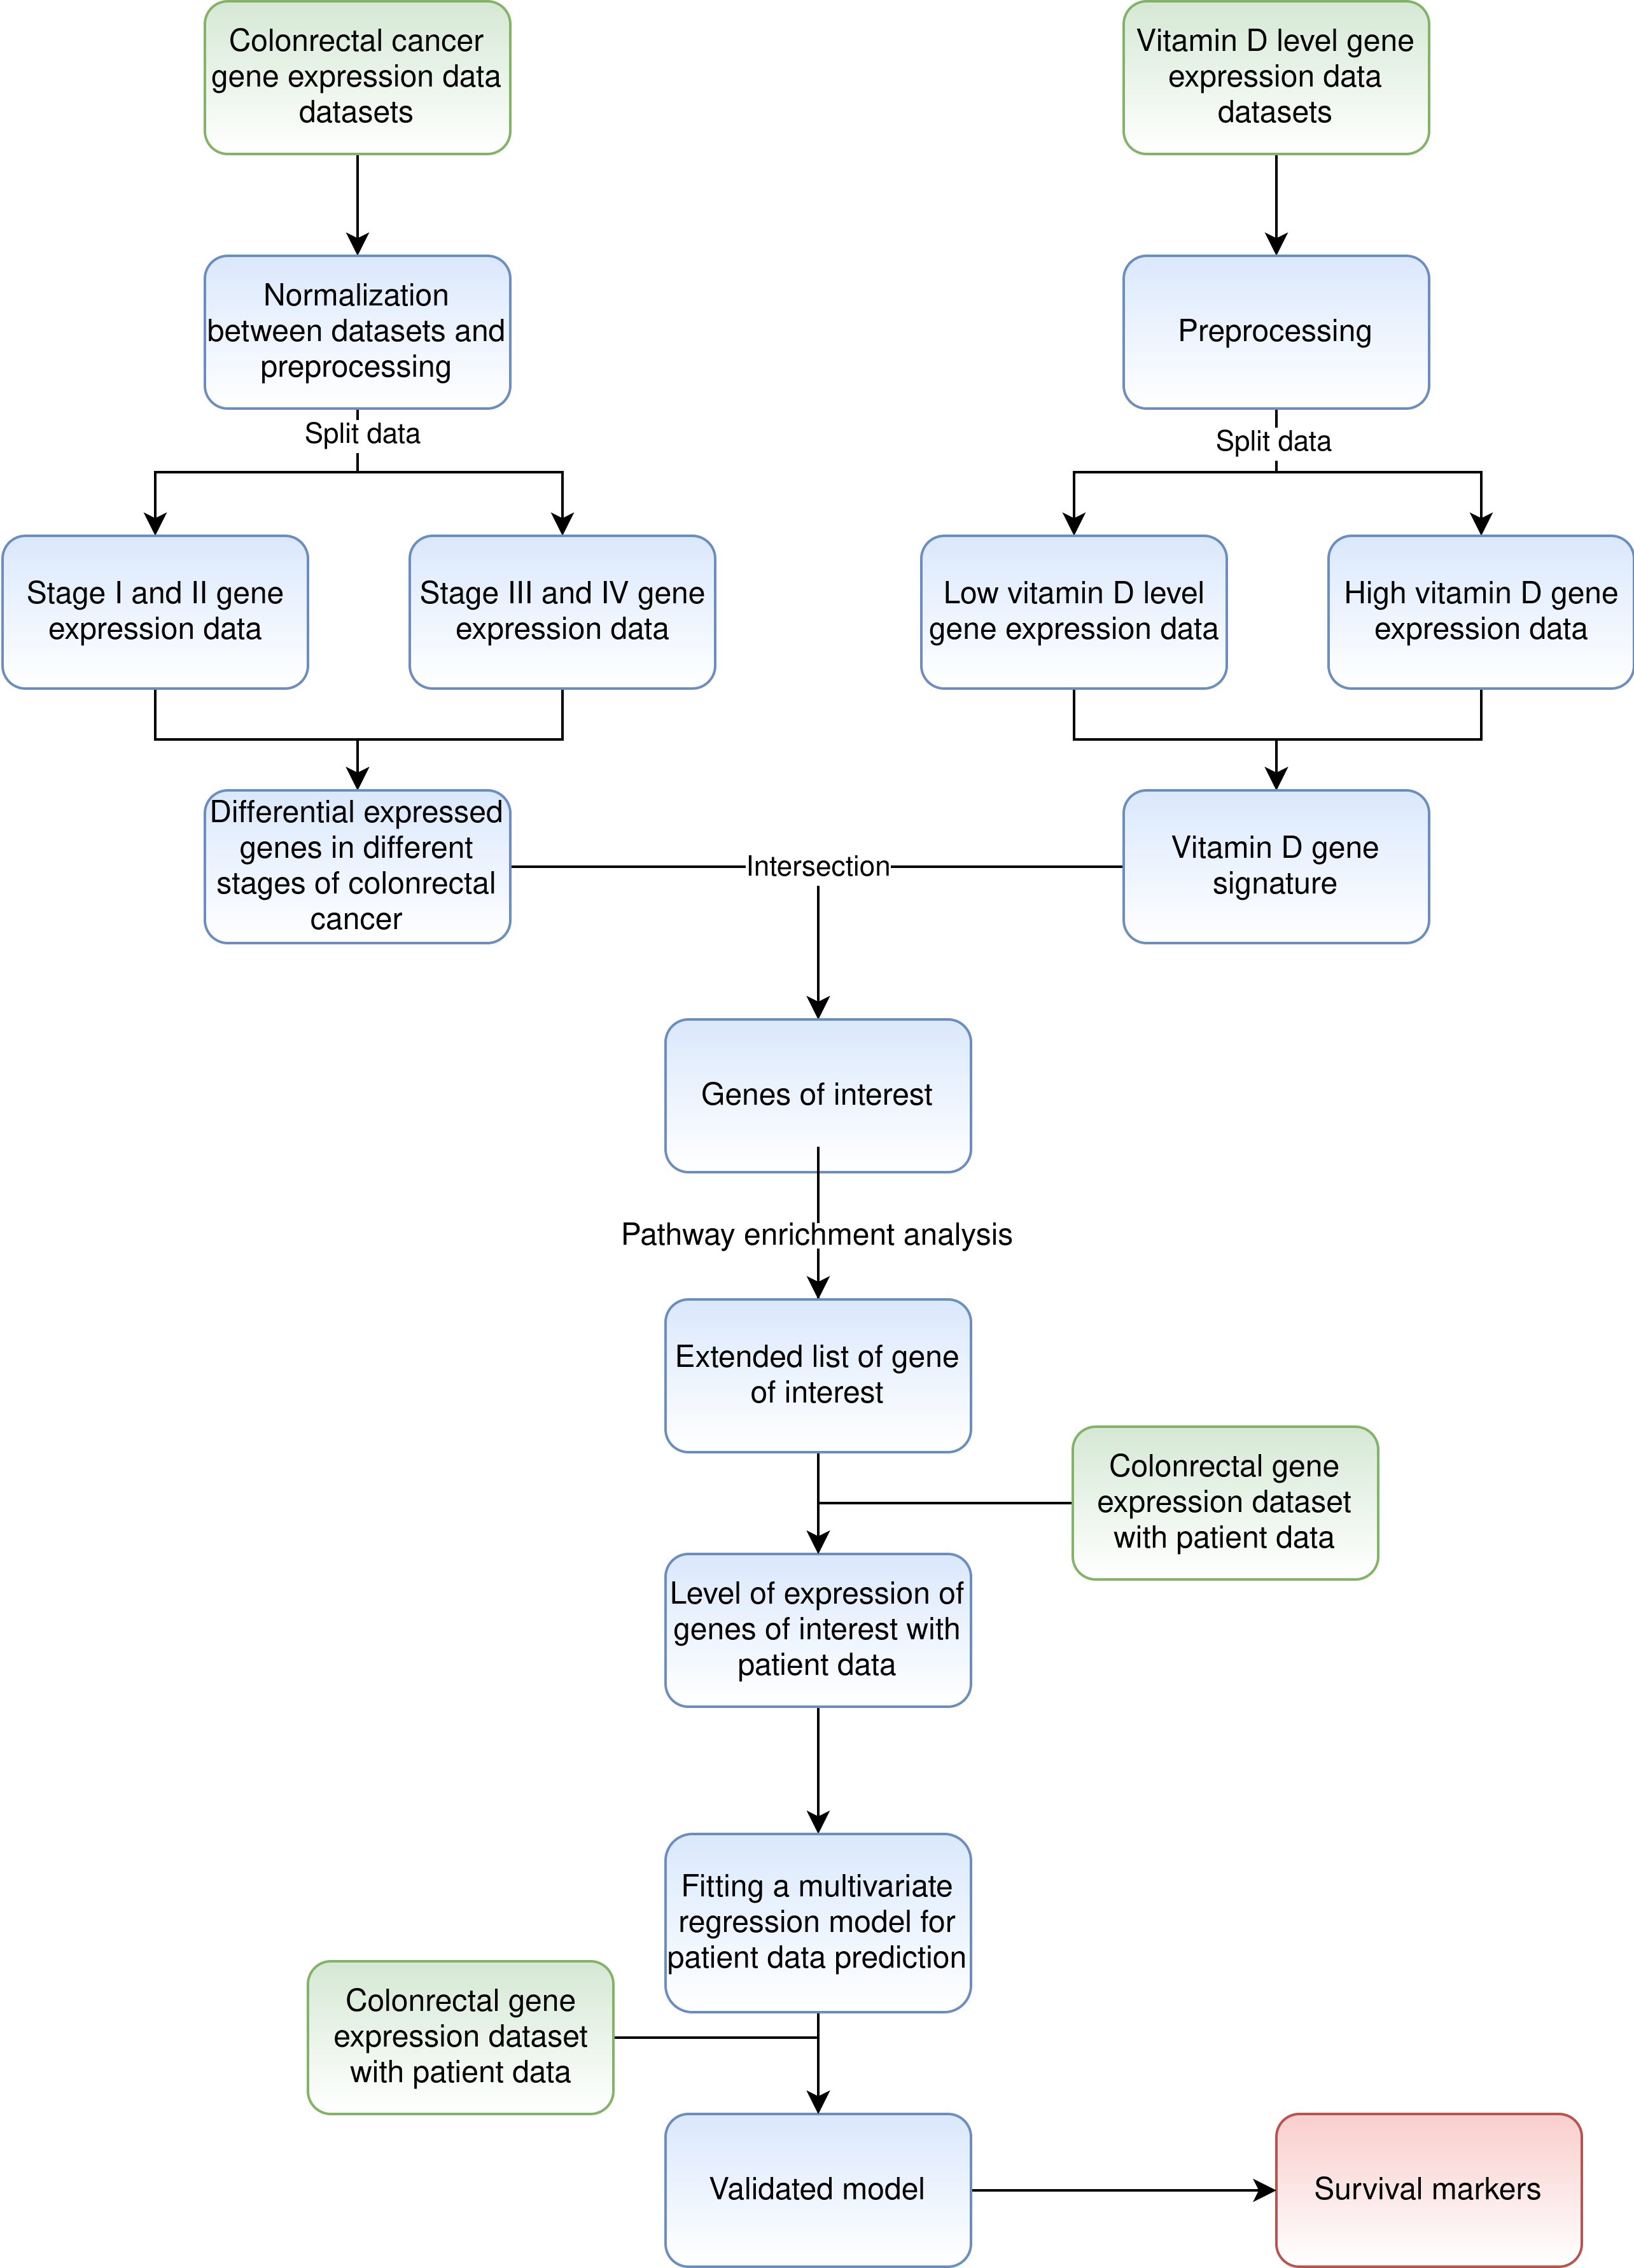
\includegraphics[width=\linewidth]{pipeline}
	\caption{Project pipeline}
	\label{fig:pipeline}
\end{figure}

	\subsection{Data pre-processing}

		\subsubsection{Normalization}
		This pipeline requires lots of samples, so we are retrieving them from different datasets.
		Because of this a normalization step is necessary: the batch effect could affect the accuracy of our predictions introducing noise in the data.
		We will try to normalize the data using different algorithms and evaluate them so to use the one that will leave the least noise.

		\subsubsection{Data filtering}
		After normalization we will filter out samples without survival data or with non-comparable data distribution.

		\subsubsection{Evaluation of pre-processed data}
		The evaluation can be done using PCA, linear regression or hierarchical cluster analysis.

	\subsection{Obtaining the list of gene of interest}

		\subsubsection{Differentially expressed genes between different stages of CRC}
		Input gene expression data will be divided in "stage I and II" and "stage III and IV", in order to obtain DEGs in different stages of colorectal cancer.


		\subsubsection{Vitamin D gene signature in CRC}
		Input gene expression data will be divided in "low vitamin D level" and "high vitamin D level", in order to obtain vitamin D gene signature.


		\subsubsection{Intersection and enrichment}
		Obtained lists of DEGs and vitamin D gene signature will be intersected in order to obtain a subset of genes of interest. On these we will then perform a pathway enrichment analysis.

	\subsection{Fitting to a regression model}
		After that, these data will be used to fit a regression model in order to assess for each gene of interest its correlation with the stratification of the patient.

	\subsection{Obtaining the survival markers}
	After model fitting the list of genes will be reduced so that it contains only genes with a significative prognostic power on patient stratification.

\section{Expected results}
With this project we expect to identify a list of genes usable as survival markers for colorectal cancer.
A list of putative genes identified in literature \cite{Bu2021-we} \cite{Ferrer-Mayorga2017-dv} \cite{Martinez-Romero2018-gp} \cite{Wang2020-mr} is displayed in table \ref{tab:suvmark}.

\begin{table}[ht]
	\centering
	\begin{tabular}{cc}
		\hline
		Gene & \\
		\hline
		CYP24A1 & \makecell{Cytochrome P450 Family 24 Subfamily \\A Member 1 Solute Carrier Family 10 \\Member 2}\\

			TGFB1 &\makecell{Transforming Growth Factor Beta\\ 1 Solute Carrier Family 10 \\Member 2}\\

			IGFBP2 &\makecell{Insulin Like Growth Factor Binding\\ Protein 2 Solute Carrier Family 10 \\Member 2} \\

			CH25H &\makecell{Cholesterol 25-Hydroxylase Solute\\ Carrier Family 10\\ Member 2} \\

			IGFLR1 &\makecell{IGF Like Family Receptor 1 Solute\\ Carrier Family 10\\ Member 2}\\

			PTPN14 &\makecell{Protein Tyrosine Phosphatase Non-Receptor\\ Type 14 Solute Carrier Family 10\\ Member 2}\\

			SLC10A2 &  \makecell{Solute Carrier\\ Family 10\\ Member 2}\\

			FGF2 &\makecell{Fibroblast Growth Factor 2\\ Solute Carrier Family 10\\ Member 2}\\
		\hline
	\end{tabular}
	\caption{Putative Vitamin-D -related CRC prognostic marker genes}
	\label{tab:suvmark}
\end{table}

\section{Project management}
The project will be developed in a dynamic and teamwork driven manner.
This is done in order to be able to leverage the particular skills and knowledge of each member.
Each task will be divided into the members in subtasks tailored according to their background.
Time estimates for each part are outlined in the following Gantt chart.
\begin{figure}[ht]
	\label{gantt}

	\begin{ganttchart}[
		vgrid,
		title label font = \tiny,
		inline,
		time slot format=isodate,
		x unit=2mm,
		canvas/.style= { fill = green!25, draw =green!50, thick},
		bar/.append style={fill=red!50},
		title/.style={fill=yellow!50}
		]{2021-11-08}{2021-12-12}
		\gantttitlecalendar{month, day, week=1, weekday} \\
	\ganttbar{\makecell{Dataset \\normalization}}{2021-11-08}{2021-11-11}\\
	\ganttbar{\makecell{Normalization\\Evaluation}}{2021-11-12}{2021-11-18}\\
	\ganttbar{\makecell{Obtaining\\ DEGs}}{2021-11-19}{2021-11-22}\\
	\ganttbar{\makecell{Obtaining \\Vitamin D \\gene signature}}{2021-11-19}{2021-11-22}\\
	\ganttbar{\makecell{Pathway \\analysis}}{2021-11-22}{2021-11-28}\\
	\ganttbar{\makecell{Model selection \\ and fitting}}{2021-11-29}{2021-12-05}\\
	\ganttbar{\makecell{Model \\validation}}{2021-12-06}{2021-12-10}\\
	\ganttbar{\makecell{Survival\\ markers\\ analysis}}{2021-12-11}{2021-12-12}\\
	\end{ganttchart}
\end{figure}
%------------------------------------------------

%----------------------------------------------------------------------------------------
%	REFERENCE LIST
%----------------------------------------------------------------------------------------
\phantomsection
\bibliographystyle{unsrt}
\bibliography{references.bib}

%----------------------------------------------------------------------------------------

\end{document}
